% This is a template for doing homework assignments in LaTeX
% !TeX TXS-program:bibliography = txs:///biber
\documentclass{article} % This command is used to set the type of document you are working on such as an article, book, or presenation

\usepackage{geometry} % This package allows the editing of the page layout
\usepackage{amsmath}  % This package allows the use of a large range of mathematical formula, commands, and symbols
\usepackage{graphicx}  % This package allows the importing of images
\usepackage{algorithm2e}
\usepackage{amsfonts} 
\usepackage{graphicx}
\usepackage{makecell}
\usepackage{verbatim}
%\usepackage{mathtools}
%\usepackage{mathabx} 
%\usepackage{float}
\usepackage{subcaption}
%\usepackage[caption = false]{subfig}
\usepackage[nottoc]{tocbibind}
% In order to get bibtex running:
% https://howtoinstall.co/en/texlive-bibtex-extra
% youtube video on compiling latex in vscode
% https://www.youtube.com/watch?v=QK_yc9qSa2w
\title{Training dataset size prediction when adopting image counts individually per class.}
\author{Thomas Mühlenstädt}

\graphicspath{ {./plots/} }
\RestyleAlgo{ruled}

%
\newcommand{\nosemic}{\SetEndCharOfAlgoLine{\relax}}% Drop semi-colon ;
\newcommand{\dosemic}{\SetEndCharOfAlgoLine{\string;}}% Reinstate
\newcommand{\pushline}{\Indp}% Indent
\newcommand{\popline}{\Indm\dosemic}% Undent
%

\begin{document}
\maketitle

\section*{Abstract}

To be added at the end.

\section{Introduction}

To be added at the end.


\section{relevant literature}
The authors of \cite{mahmood2022data} go beyond estimation of data set requirements from power law function and investigate three alternative regression functions i.e. Arctan, Logarithmic, Algebraic Root. They show that all of the functions are well-suited towards estimating model performance however each function is almost always either overly optimistic i.e. under-estimating the data requirement or pessimistic i.e. over-estimating. This means that there is no one best regression function for all situations. Through simulation of a data collection workflow the paper shows that incrementally collecting data over multiple rounds and combining those with techniques that under-estimate leads to collecting up to 90\% of the true amount of data needed. In addition the authors introduce a correction factor that can be learned by simulating on prior tasks and which helps to better fitting functions. The fitting of the three regression functions and the benefits of the usage of the correction factor have been applied on classification, detection, and segmentation tasks with different data sets incl. CIFAR10.

The paper \cite{cho2016data} focuses on predicting the needed training dataset size for achieving necessary accuracy for a classification task in the medical domain. More precisely the use case is classifying axial Computed Tomography (CT) images into six anatomical classes. The authors apply the already introduced (\cite{Figueroa2012PredictingSampleSizeForClass}) power law fitting to the mentioned use case. This paper focuses only on the medical domain and provides among the first empirical results that the power law fitting for determining the training data set size also applies for the medical domain.

Inspired by the fact that power law scaling of the error w.r.t. data suggests that many training examples are redundant, the authors of \cite{sorscher2023neural} investigate the hypothesis of pruning training datasets to much smaller sizes and training on the smaller pruned datasets without sacrificing performance. The authors show in theory and in practice that one can break beyond power law scaling and even reduce it to exponential scaling if one uses an efficient data pruning metric that ranks the order in which training examples are being discarded. The theory proof reveals two very interesting points: 1) the optimal pruning strategy changes depending on the amount of initial data i.e. with abundant (scarce) initial data, one should retain only hard (easy) examples and 2) exponential scaling is possible w.r.t. pruned dataset size only if one chooses an increasing Pareto optimal pruning fraction as a function of initial dataset size. The authors demonstrate empirically the exponential scaling of the error w.r.t. pruned dataset size for a ResNets trained from scratch on SVHN, CIFAR-10 and ImageNet, and Vision Transformers fine-tuned on CIFAR-10. In addition, the paper presents a new and comparably good unsupervised data pruning metric that does not require labels, unlike other prior unsupervised pruning metrics that require labels and much more compute. The k-means based pruning metric (clustering in the embedding space of an ImageNet pre-trained model) enables discarding of 20\% of ImageNet data without sacrificing performance, on par with the best and most compute intensive supervised metric.

Motivated by the fact that GPUs and model capacity have continuously continued to grow, but training datasets have remained stagnant, the authors of \cite{sun2017revisiting} investigate the impact of big datasets (i.e. the JFT-300M) on the performance of vision tasks (e.g. object detection, segmentation etc. ). The JFT dataset contains more than 300M images that are labeled with 18291 annotations and the authors use the ResNet-101 model architecture in the experiments. The experiments show that performance increases logarithmically based on the volume of training data. This is valid for both use cases i.e. when using fine-tuning and when using freezing feature extractors. The authors perform also further experiments in which they show couple of more interesting findings e.g. 1) capacity is crucial i.e. in order to fully use the 300M images, one needs higher capacity models. For example, in case of ResNet-50 the gain on COCO object detection is much smaller (1.87\%) compared to (3\%) when using ResNet-152. 2) JFT-300M has 18K labels in total and in order to understand what the large number of classes brings, the authors select a subset of 941 labels which have direct correspondence to the 1000 ImageNet labels. The experiments show that performance benefit comes from more training images instead of more labels.

Compared to the other papers that mainly target vision tasks \cite{hoffmann2022training} focus on large language model. The trend so far in large language model training has been to increase the model size, often without increasing the number of training tokens. Thus the paper investigates the optimal model size and number of tokens for training a transformer language model under a given compute/FLOPs budget. The paper presents three predictive approaches that start by training a range of models varying both model size and the number of training tokens and use the resulting training curves to fit an empirical estimator. Similarly as some of the above presented literature the paper assume a power-law relationship between compute and model size. The resulting predictions are similar for all three methods and suggest that parameter count and number of training tokens should be increased equally with more compute i.e. for every doubling of model size the number of training tokens should also be doubled. The authors propose and use the Chinchilla LLM to test and proof the hypothesis.

The authors of \cite{alabdulmohsin2022revisiting} revisit the scaling law in vision and language domain and emphasise that in order to achieve benefits of such scaling laws in practice, it is important that scaling laws extrapolate accurately instead of interpolating the learning curve. The paper shows how the scaling exponent c of a power law estimator that extrapolates best can be quite different from the exponent that best fits the given (finite) learning curve. Thus a new estimator (denoted as M4) is proposed which extrapolates more accurately than previous methods such as a power law estimator M2. M2 is a subset of M4 such that using M4 becomes equivalent to using M2 when the observed learning curve resides entirely in the power law regime. Moreover, the M4 estimator has a sigmoid shape and that contributes to the better performance. The new proposed estimator M4 has been validated in several domains such as image classification, neural machine translation, language modelling, and other related tasks. For the validation the authors propose a more rigorous validation of scaling law parameters based on the extrapolation loss.

Compared to the previous mentioned papers where the scaling law has been empirically determined for a diverse of problem types (supervised, unsupervised, transfer learning) and data types (images, video, text, ) and many NN architectures (Transformers, ConvNets, ...), \cite{hutter2021learning} focuses on the theoretical understanding of the phenomena (error scaling w.r.t. data size n). In finite-dimensional models, the error typically decreases with n - 1/2 or n - 1 , where n is the sample size. ...

\cite{hoffmann2022training}
\cite{alabdulmohsin2022revisiting}
\cite{hutter2021learning}
\cite{mahmood2022data}
\cite{rosenfeld2019constructive}
\cite{sorscher2023neural}
\cite{sun2017revisiting}
\cite{cho2016data}

\begin{itemize}
    \item https://arxiv.org/pdf/2203.15556.pdf
    \item https://arxiv.org/pdf/2207.01725.pdf
    \item https://arxiv.org/pdf/2206.14486.pdf
    \item https://arxiv.org/pdf/2209.06640.pdf
    \item https://arxiv.org/pdf/2102.04074.pdf
    \item https://arxiv.org/pdf/1909.12673.pdf
    \item https://arxiv.org/pdf/1707.02968.pdf
    \item https://arxiv.org/abs/1511.06348
    \item Baidu paper?
\end{itemize}

\section{Overview suggested method}

The task considered here is image classification, i.e. we aim to find a model $y = f_{\theta}(x)$, where $x$ is an image tensor and $y$ being a one hot encoding for the classes contained in the dataset.
The training data consists of $k$ classes, which each class $j$ having $n_j^{max}$ labeled images in the training dataset with $n^{max} = \sum_{j= 1}^k n_j^{max}$ being the overall number of training images.
Also, for completeness, we assume there is a labelled test and/or validation data set used to calculate the performance of a trained model $f_{\hat{\theta}}(x)$.
The performance metric we are using here is accurcy, denoted as $a(f_{\hat{\theta}}(.))$. But in general, the methods described here would also for other metrics like e.g. $f_1$ scores, precision or recall.
We refer to standard literature like e.g. \cite{Goodfellowetal2016} and \cite{Bishop2006PatternRecog} for these general details.
Most of the literatur for neural scaling laws focusses on assuming different training dataset sizes $n^{train}$ for a number of different training jobs, i.e. to find a function $g_{\omega}(n^{train})$ which can predict the chosen performance metric for different training dataset sizes.
This means implicitely that each class has the same importance for the performance.
But this is not necessarily true, some classes might be more difficult to train on than others.
Hence here an approach is taken, which allows to estimate the importance of training images from each class individually.
Also, the compute budget is an important aspect of performance, hence we also aim at considering how different number of training epochs affects performance.
Hence, we are aiming at expanding the function $g_{\omega}(n^{train})$ to be more general: $g_{\omega}(n_1^{train}, \dots, n_k^{train})$ shall be a function predicting the performance of our model depending on the individual class training image counts.
Even more general, we can also incorporate the number of training epochs $n^{epoch}$ used for estimating the parameters $\theta$ into the function, now becoming $g_{\omega}(n_1^{train}, \dots, n_k^{train}, n^{epoch})$.
In order to fit functions which allow for estimation of more differentiating effects between classes and epochs, more divers training datasets need to be generated.
Hence one focus of this paper is to suggest an algorithm which allows for generation of divers training data sets.
For modeling these data and making predictions and importance statements, non-linear models like powerlaw curves are fitted in a way that the input is a linear combination of the training dataset size per class plus the number of epochs trained.
The coefficients of this linear combination are the parameters to be estimated.

\section{Data generation algorithm}

%https://core.ac.uk/reader/217880230

%https://www.jmp.com/support/help/en/17.1/index.shtml#page/jmp/references-5.shtml#


For a given training dataset, a smaller subset can sampled randomly by assigning the same probability of being included in the sample to each image.
Although in general this is a good sampling strategy in many contexts, here it is not what is desired.
Especially for large training datasets, the law of large numbers says that the class proportions in the sample subset will be very similar to the class distribution in the complete training dataset.
In order to achieve a number of divers training datasets, both with respect to the total size as well with respect to the class proportions, an algorithm is suggested in the following.
It takes some motivation from a special case of statisticial design of experiments, notably constrained space filling mixture designs. Please see \cite{gomes_hal_spacefilling_mixtures} for more information on spacefilling mixture desigsn.
Design of experiments is a set of methods, originating back to as early as Sir Ronald Fishers book on the topic \cite{fisher_1935}, which all aim at collecting optimal data for fitting a specific statistical/mathematical model. This might be simple linear models (cite something) or much more complex
models like nonlinear, multidimensional models \cite{myers2009response}, \cite{Goos_Jones_optDoE_2011}. In contrast to many machine learning and active learning methods, design of experiments
often aims at finding the minimal dataset with which a model can be fitted.
Mixture designs in general are a class of designs originating out of chemistry: The composition of some ingredients to a chemical experiments needs to sum up to 100\%, see for example \cite{Nist_2012_eng_stats}, chapter 5.5.4 for a short introduction.
The reason why this is fitting here is that, given a target dataset size $n_{subset}$, we want to create a number of different combinations of training datasets, which all have the same total number of training images but distributed differently according to the different classes.
There are different ways to describe the optimality of a design of experiments. Here we will choose an optimality criterion which is considered space filling, the so called maximin optimality criterion, which tries to maximize the minimum (euclidean) distance between any two data points in the design.
The reasoning behind this is that having a datapoint $d_2 \in D$ , which are very close to a datapoint $d_1 \in D$ does not bringing additional benefit, as we have learned already the response of
our target function $g(.)$ at position $d_1$.
This choice is to a big degree subjective. We have chosen this optimality criterion here, as we want to generate a wide spread of different combinations of class counts, given a fixed overall count of training images.
The design needs to be constrained, as for larger subset sizes, it might happen that a purely randomly generated combination of class counts is for some classes higher than the maximum number of available training images per class.
The algorithm to find an optimal design has 2 stages: In the initilization phase, a design is constructed which is fullfilling the following: each row summing up to the target dataset size and the constraint for the maximum number of images per class is full filled.
In the second stage, this design is improved iteratively by a pointwise exchange algorith: The pair of design points with the minimal distance is found and one of them is replaced by a new, randomly generated candidate design point.
If the maximin criterion for the new candidate design is improved compared to the previosly best design, the candidate design is accepted as new best design.
Otherwise, the candidate design is rejected. This process is repeated a fixed number of times.
Similar pointwise optimization procedures are quite common in the area of design experiments and are rooting back to early references like \cite{fedorov1972theory}.
One important detail in this process is how design points are suggested, during the initialization phase as well as during the optimization phase.
For the unconstrained case, candidate points can be suggested by using TBD. In the case of heavliy constrained mixture, a heuristc can be applied to increase the chance to sample a candidate fullfilling the constraint. For details, please check in the appendix.



\begin{algorithm}
    \SetKwInOut{Input}{input}\SetKwInOut{Initialize}{initialize}\SetKwInOut{Optimize}{optimize}
    \caption{Mixture Design creation} \label{alg:one}
    \nosemic
    \Input{\;
        \dosemic
        \pushline
        Define $n_{doe} \in \mathbb{N}$: The number of rows to be generated\;
        Define $n_{cmax} \in \mathbb{N}$: The maximum number of training images in each class\;
        Define $n_{opt} \in \mathbb{N}$: The maximum number of iterations used for optimizing the DoE\;
        Define $n_{candidate} \in \mathbb{N}$: The batch size for generating candidate mixture datapoints\;
    }
    \Initialize{\;
        \dosemic
        Intialize $\tilde{doe}$ as empty dataframe\;
        Set $n_{doe} = 0$\;
        \While{$\tilde{n}_{doe} < n_{doe}$}{
            Create a batch of candidate mixture datapoints $candidates$ of size $n_{candidate}$\;
            For each candidate point: Delete candidate point, if for any class $c$ $n^{c} > n_{cmax}$\;
            Add all remaining rows of $candidates$ to $\tilde{doe}$\;
            set $n_{doe} = $ number of rows of $doe$ \;
        }
        Set $doe$ to the first $n_{doe}$ rows of $\tilde{doe}$\;
    }
    \Optimize{\;
        \dosemic
        Set $doe_{opt} = doe$\;
        Set $Mm = \min_{t \neq b}(\|x_t - x_b\|)$ \;
        \For{$i \leq n_{opt}$}{
            Set $\tilde{doe} = doe_{opt}$\;
            Determine point pair $k \neq j$ with $\|x_k - x_j\| = \min_{x_t \neq x_b \in \tilde{doe}}(\|x_t - x_b\|) $\;
            Create a candidate point $\tilde{x}$ with $max(x^{c}) \leq n_{cmax}$ (fullfilling class constraints)\;
            In $\tilde{doe}$, replace point $x_k$ with $\tilde{x}$\;
            \If{$\min_{x_t \neq x_b \in \tilde{doe}}(\|x_t - x_b\|) > Mm$}{
                Set $doe_{opt} = \tilde{doe}$\;
                Set $Mm = \min_{x_t \neq x_b \in \tilde{doe}}(\|x_t - x_b\|)$\;
            }
        }
    }
\end{algorithm}





\begin{algorithm}
    \SetKwInOut{Input}{input}
    \caption{Data generation}\label{alg:two}
    \nosemic
    \Input{ \;
        \dosemic
        \pushline
        Choose an image classification dataset\;
        Choose a network architecture $f_{\theta}(x)$ suitable for the chosen image classification\;
        Define a sequence $subsets$ of growing integers between $0$ and $n_{train-max}$\;
        Define $n_{repeat} \in \mathbb{N}$: The number of rows to be generated per $s \in subsets$\;
        Define $e_{max} \in \mathbb{N}$: The maximum number of epochs to train a network \;
        Define a sequence $e_{check}$ with elements $c \in \mathbb{N}, c \le e_{max}$: The epochs where to evaluate performance of
    }
    \For{$s \in subsets$}{
        Generate mixture design $D_s$ for subset size $s$ with $n_{repeat}$ rows\;
        \For{$i \in (0, \dots,  n_{repeat} - 1)$}{
            Generate training dataset $T_{i, s}$according to row $D_{s, i}$\;
            Initialize network $f_{\theta}$\;
            \For{$e \in (0, \dots, e_{max})$}{
                Train network $f_{\theta}$ for one epoch\;
                \If{$e \in check_e$}{
                    Evaluate the performance of $f_{\theta}$ on the test dataset\;
                    Write the evaluation results (losses, metrics) to a logger\;
                }
            }

        }
    }
\end{algorithm}


\section{scaling law model fitting}

\begin{itemize}
    \item Power law scaling (\cite{mahmood2022data}): $g_{\omega}(n) = \omega_1 n^{\omega_2} + \omega_3$.
    \item Arctan scaling: $g_{\omega}(n) = \frac{200}{\pi} \arctan(\omega_1 \frac{\pi}{2}n + \omega_2) + \omega_3$
    \item logarithmic scaling: $g_{\omega}(n) = \omega_1 \log(n + \omega_2) + \omega_3$
    \item Algebraic root: $g_{\omega}(n) = \frac{100n}{1 + \| \omega_1 n\|^{1/\omega_2}} + \omega_3$
    \item For each of these models, we can replace $n$ by a linear combination of $n_c$, the class counts: $n$
    \item Another model class used here is a logistic regression, as this naturally expands from a one dimensional (i.e. just using the overall training dataset size $n$) to the multidimensional use case (Using seperate class counts).
\end{itemize}

\section{Experiments using CIFAR10}

\subsection{experimental setup}
The CIFAR10 dataset \cite{Cifar10} is a well known benchmark dataset for image classification.
It consists of 50000 training images, in 10 classes, each class having 5000 training images of the shape 32x32x3 and 10000 test images of the same shape, also equally distributed across the 10 classes.
As a model to be fitted, a standard Resnet18 architecture \cite{he2015resnet} has been used as standard model here, as implemented in the pytorch \cite{pytorch} modell zoo.
For optimizing this model, a standard SGD optimizer with cross entropy loss has been used with $learning_rate = 0.1, momentum=0.9$ and $weight_decay=1e-4$, together with a learning rate scheduler, reducing the the learning at 100 (which is also clearly visible at severals accuracy vs. epoch plots, e.g. Figure \ref{fig_full_dataset_epoch_vs_acc}) and 150 epochs.
For data preparation/transformations, random horizontol flipping, random cropping and batch normalization with predefined mean and standard deviation  has been used.
With these settings, validation dataset accuracies up to 84\% have been achieved.
There are for sure more advanced model architectures for the Cifar10 dataset, however we aimed at balancing an at least medium performant model with a having a reasonable training time, as the training process is repeated here a high number of times.
For the experiemtns done here, we applied the algorithm from section 4 here with the following settings:
As subset sizes we have chosen $[5000, 10000, \dots, 40000, 45000]$. For each subset size a design of experiments according to Algorithm \ref{alg:two} with 30 different settings has been created for training a function $g_{\omega}$ as well as a validation dataset with 15 runs per subset size.
For each training dataset, the same model and hyperparameter settings has been used, training for up to 195 epochs, checking for validation accuracy every 5 epochs.
To get an impression of the models fitted here, there are a number of descriptive visulizationas in Figures \ref{fig_full_dataset_epoch_vs_acc}, \ref{fig_traing_subset_size_vs_test_acc} and \ref{fig:accuracy_vs_epoch_by_subset_size}. In Figure \ref{fig_full_dataset_epoch_vs_acc} the test set accuracy for the full training dataset across different epochs and 10 repeats is shown.
In Figure \ref{fig_traing_subset_size_vs_test_acc} the test accuracy at 195 training epochs for all created training dataset of different size is plotted. As expected, the performance varies more for smaller total training dataset sizes compared to larger training dataset sizes.
And in Figure \ref{fig:accuracy_vs_epoch_by_subset_size}, the test accuracy is plotted over training epoch for all training datasets of 4 different training dataset sizes.
Overall, the descriptive analysis did not yield any concerns in terms of outliers or unexpected behavior of the data.
\subsection{model fitting results}



\begin{figure}
    \begin{subfigure}{.5\textwidth}
        \centering
        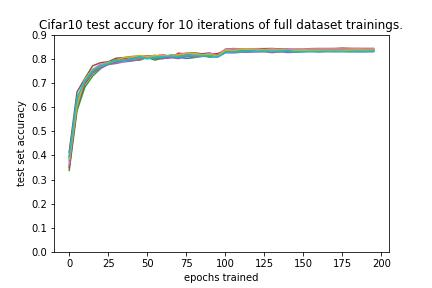
\includegraphics[width=.8\linewidth]{Cifar10_full_dataset_acc_vs_epoch}
        \caption{Full training results for 10 seperate training runs.}
        \label{fig_full_dataset_epoch_vs_acc}
    \end{subfigure}%
    \begin{subfigure}{.5\textwidth}
        \centering
        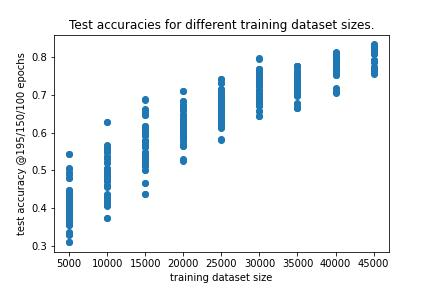
\includegraphics[width=.8\linewidth]{Cifar10_training_datasetsize_vs_test_acc}
        \caption{Test accuracies vs. training dataset sizes.}
        \label{fig_traing_subset_size_vs_test_acc}
    \end{subfigure}

    \caption{Descriptive results for the models fitted to Cifar10 dataset.}
    \label{fig:desc_plots_cifar10}
\end{figure}



\begin{figure}
    \begin{subfigure}{.5\textwidth}
        \centering
        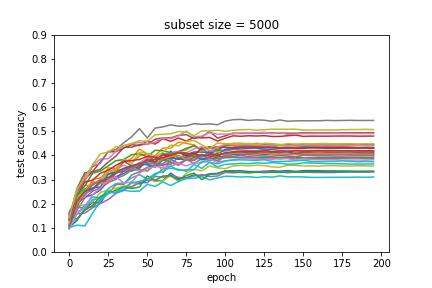
\includegraphics[width=.8\linewidth]{test_acc_vs_epoch_subset_size_5000}
        \caption{training dataset size = $5000$ images}
        \label{fig:subsetsize5000}
    \end{subfigure}%
    \begin{subfigure}{.5\textwidth}
        \centering
        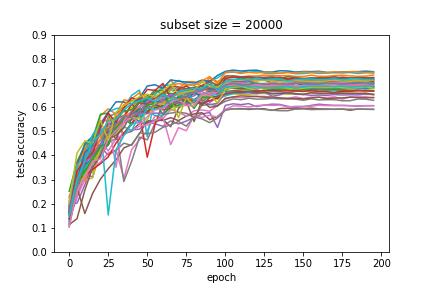
\includegraphics[width=.8\linewidth]{test_acc_vs_epoch_subset_size_20000}
        \caption{training dataset size = $20000$ images}
        \label{fig:subsetsize20000}
    \end{subfigure}
    \begin{subfigure}{.5\textwidth}
        \centering
        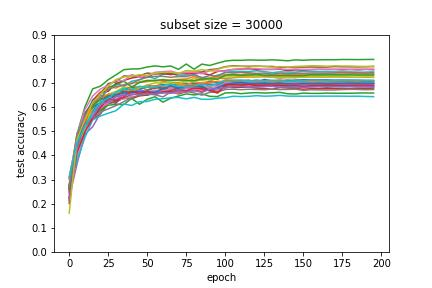
\includegraphics[width=.8\linewidth]{test_acc_vs_epoch_subset_size_30000}
        \caption{training dataset size = $30000$ images}
        \label{fig:subsetsize30000}
    \end{subfigure}%
    \begin{subfigure}{.5\textwidth}
        \centering
        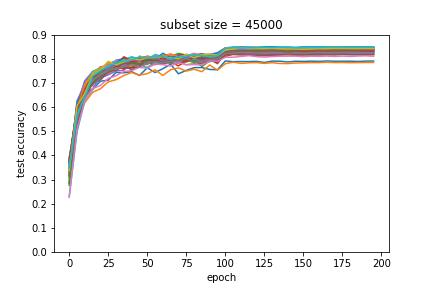
\includegraphics[width=.8\linewidth]{test_acc_vs_epoch_subset_size_45000}
        \caption{training dataset size = $45000$ images}
        \label{fig:subsetsize45000}
    \end{subfigure}

    \caption{Test accuracies vs. epochs for different number of training dataset sizes.}
    \label{fig:accuracy_vs_epoch_by_subset_size}
\end{figure}

\begin{table}[h!]
    \centering
    \begin{tabular}{|r|c|c|c|c|c|c|}
        \hline
        short description   & no  & linear combination                               & train loss & test loss & train acc $r^2$ & test acc $r^2$ \\
        \hline
        full model          & $0$ & $\beta_e x_{epoch} + \sum_{i = 1}^c \beta_c n_c$ & 0.00252    & 0.00262   & $87.8\%$        & $87.4\%$       \\
        \hline
        \makecell{full model                                                                                                                     \\ epoch squared} & $1$& $\beta_e x_{epoch} +\beta_{e^2} x_{epoch}^2 + \sum_{i = 1}^c \beta_c n_c$& 0.00203 & 0.00212 & $90.1\%$ & $89.8\%$ \\
        \hline
        $total_n$ and epoch & $2$ & $\beta_e x_{epoch} + \beta_n n_{total}$          & 0.00262    & 0.00251   & $87.2\%$        & $87.9\%$       \\
        \hline
        \makecell{$total_n$ and                                                                                                                  \\epoch squared} &$3$& $\beta_e x_{epoch} +\beta_{e^2} x_{epoch}^2+ \beta_n n_{total}$ & 0.00259 & 0.00249 & $87.4\%$ & $88.0\%$ \\
        \hline
    \end{tabular}
    \caption{Powerlaw model overview.}
    \label{table:model_overview}
\end{table}

\begin{table}[h!]
    \centering
    \begin{tabular}{|c|c|c|c|c|c|c|c|c|c|c|c|c|c|c|}
        \hline
        a     & b    & c    & plane & car  & bird & cat  & deer & dog  & frog & horse & ship & truck & epoch & epoch**2 \\
        \hline
        -0.18 & 0.39 & 0.58 & 0.44  & 0.38 & 0.36 & 0.21 & 0.36 & 0.33 & 0.36 & 0.45  & 0.28 & 0.30  & 2.46  & -1.79    \\
        \hline
    \end{tabular}
    \caption{Estimated parameters for model (1).}
    \label{table:param_values_full_model_epoch_sq}
\end{table}

\begin{table}[h!]
    \centering
    \begin{tabular}{|c|c|c|c|c|c|c|c|c|c|c|c|c|c|}
        \hline
        a     & b    & c    & plane & car  & bird & cat  & deer & dog  & frog & horse & ship & truck & epoch \\
        \hline
        -0.05 & 0.40 & 0.55 & 0.37  & 0.31 & 0.29 & 0.17 & 0.30 & 0.27 & 0.29 & 0.37  & 0.23 & 0.25  & 0.59  \\
        \hline
    \end{tabular}
    \caption{Estimated parameters for model (0).}
    \label{table:param_values_full_model}
\end{table}

\begin{table}[h!]
    \centering
    \begin{tabular}{|c|c|c|c|c|}
        \hline
        a    & b    & c    & total\_n & epoch \\
        \hline
        0.25 & 0.61 & 0.35 & 0.48     & 1.86  \\
        \hline
    \end{tabular}
    \caption{Estimated parameters for model (3).}
    \label{table:param_values_total_n_epoch}
\end{table}

\begin{table}[h!]
    \centering
    \begin{tabular}{|c|c|c|c|c|c|}
        \hline
        a    & b    & c    & total\_n & epoch & epoch\_sq \\
        \hline
        0.28 & 0.75 & 0.41 & 0.32     & 1.50  & -0.32     \\
        \hline
    \end{tabular}
    \caption{Estimated parameters for model (4).}
    \label{table:param_values_total_n_epoch_sq}
\end{table}

\begin{figure}
    \begin{subfigure}{.5\textwidth}
        \centering
        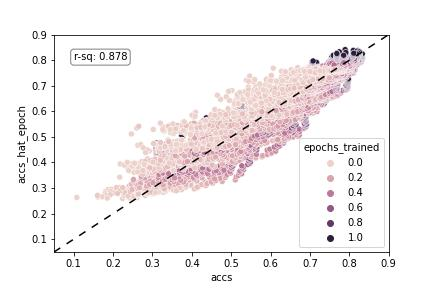
\includegraphics[width=.8\linewidth]{powerlaw_train_accs_hat_epoch}
        \caption{training dataset size = $5000$ images}
        \label{fig:powerlaw_acc_hat_epoch_train}
    \end{subfigure}%
    \begin{subfigure}{.5\textwidth}
        \centering
        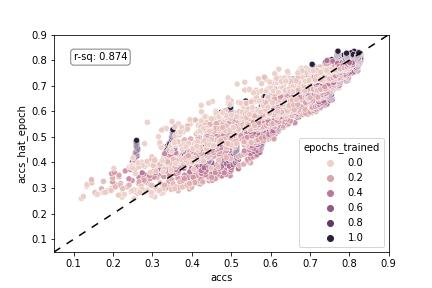
\includegraphics[width=.8\linewidth]{powerlaw_val_accs_hat_epoch}
        \caption{training dataset size = $20000$ images}
        \label{fig:powerlaw_acc_hat_epoch_val}
    \end{subfigure}
    \caption{Prediction plot for powerlaw function 0.}
    \label{fig:powerlaw_acc_hat_epoch}
\end{figure}


\begin{figure}
    \begin{subfigure}{.5\textwidth}
        \centering
        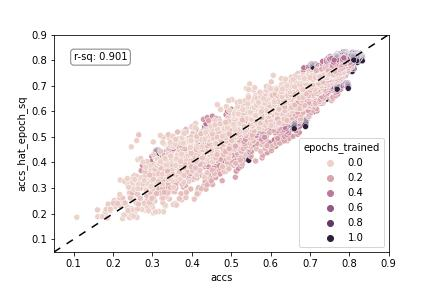
\includegraphics[width=.8\linewidth]{powerlaw_train_accs_hat_epoch_sq}
        \caption{training dataset size = $5000$ images}
        \label{fig:powerlaw_acc_hat_epoch_sq_train}
    \end{subfigure}%
    \begin{subfigure}{.5\textwidth}
        \centering
        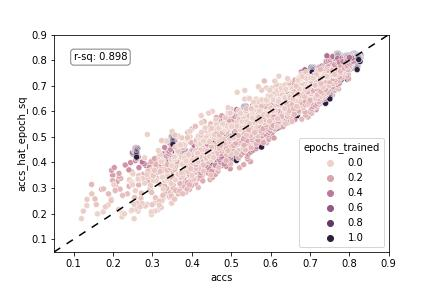
\includegraphics[width=.8\linewidth]{powerlaw_val_accs_hat_epoch_sq}
        \caption{training dataset size = $20000$ images}
        \label{fig:powerlaw_acc_hat_epoch_sq_val}
    \end{subfigure}
    \caption{Prediction plot for powerlaw function 1.}
    \label{fig:powerlaw_acc_hat_epoch_sq}
\end{figure}


\begin{figure}
    \begin{subfigure}{.5\textwidth}
        \centering
        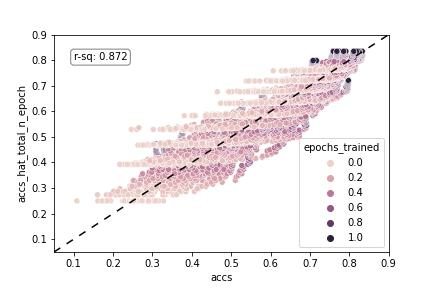
\includegraphics[width=.8\linewidth]{powerlaw_train_accs_hat_total_n_epoch}
        \caption{training dataset size = $5000$ images}
        \label{fig:powerlaw_accs_hat_total_n_epoch_train}
    \end{subfigure}%
    \begin{subfigure}{.5\textwidth}
        \centering
        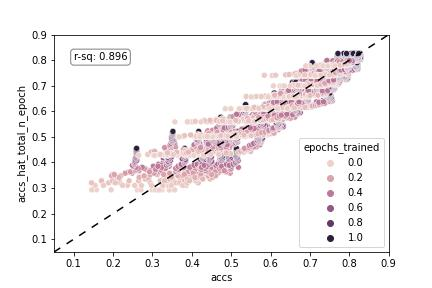
\includegraphics[width=.8\linewidth]{powerlaw_val_accs_hat_total_n_epoch}
        \caption{training dataset size = $20000$ images}
        \label{fig:powerlaw_accs_hat_total_n_epoch_val}
    \end{subfigure}
    \caption{Prediction plot for powerlaw function 3.}
    \label{fig:powerlaw_accs_hat_total_n_epoch}
\end{figure}

\begin{figure}
    \begin{subfigure}{.5\textwidth}
        \centering
        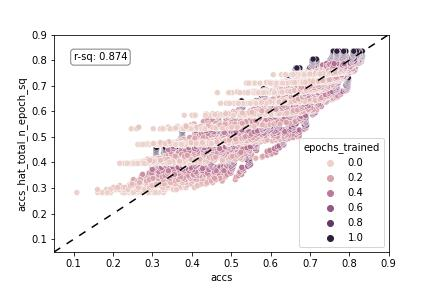
\includegraphics[width=.8\linewidth]{powerlaw_train_accs_hat_total_n_epoch_sq}
        \caption{training dataset size = $5000$ images}
        \label{fig:powerlaw_accs_hat_total_n_epoch_sq_train}
    \end{subfigure}%
    \begin{subfigure}{.5\textwidth}
        \centering
        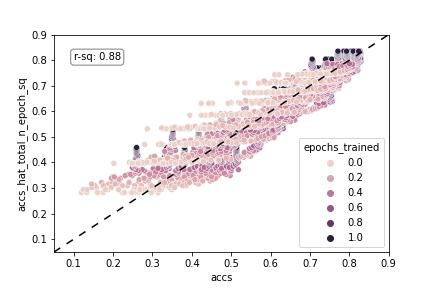
\includegraphics[width=.8\linewidth]{powerlaw_val_accs_hat_total_n_epoch_sq}
        \caption{training dataset size = $20000$ images}
        \label{fig:powerlaw_accs_hat_total_n_epoch_sq_val}
    \end{subfigure}
    \caption{Prediction plot for powerlaw function 4.}
    \label{fig:powerlaw_accs_hat_total_n_epoch_sq}
\end{figure}


\begin{itemize}
    \item In preparation for model fitting, the data have been transformed in the following way:
    \item \begin{itemize}
              \item All model results for epochs $< 10$ have been removed from the dataset. Mainly because these data are highly variable.
              \item From the individual class counts an overall training dataset size is calculated per dataset.
              \item All class counts (also the total dataset size) have been scaled to be between $[0, 1]$, as well as the epochs.
              \item As the test accuracies are already between $[0,1]$ these have not been further standardized.
          \end{itemize}
    \item Following these desecriptive plots, a number of different models are fitted, all using the above described dataset.
    \item In Table \ref{table:model_overview} an overview of the fitted models is given.
    \item All of the these models are fitted using the \verb|curve_fit| function from the python package \verb|scipy.optimize|.
    \item The resulting parameter estimates are shown in Tables \ref{table:param_values_full_model_epoch_sq} to \ref{table:param_values_total_n_epoch_sq}.
    \item For each model, there is a corresponding pair of prediction plots (one for the train data set and one for the validation dataset) in Figures \ref{fig:powerlaw_acc_hat_epoch} to \ref{fig:powerlaw_accs_hat_total_n_epoch_sq}.
    \item Looking at Table \ref{table:model_overview}, the model using the individual class counts and the epoch in a linear and squared effect performs best.
    \item Also, for this model, the prediction plots look most reasonable, scattering rather randomly around the diagonal.
\end{itemize}

\section{Discussion summary}

\pagebreak
\bibliographystyle{ieeetr}
\bibliography{lit}

\section*{Appendix}



\begin{table}[h!]
    \centering
    \begin{tabular}{lrrrrrrrrrrrrr}
        row & accs & plane & car & bird & cat & deer & dog & frog & horse & ship & truck & epochs & $total_n$ \\
        \hline
        0   & 0.18 & 145   & 31  & 97   & 496 & 1096 & 307 & 2382 & 10    & 373  & 63    & 10     & 5000      \\
        1   & 0.21 & 145   & 31  & 97   & 496 & 1096 & 307 & 2382 & 10    & 373  & 63    & 15     & 5000      \\
        2   & 0.20 & 145   & 31  & 97   & 496 & 1096 & 307 & 2382 & 10    & 373  & 63    & 20     & 5000      \\
        3   & 0.25 & 145   & 31  & 97   & 496 & 1096 & 307 & 2382 & 10    & 373  & 63    & 25     & 5000      \\
        4   & 0.24 & 145   & 31  & 97   & 496 & 1096 & 307 & 2382 & 10    & 373  & 63    & 30     & 5000      \\
    \end{tabular}
    \caption{First few lines of the underlying data table used for fitting the powerlaw models.}
    \label{table:datatable_results}
\end{table}


\end{document}
